\documentclass[a4paper]{article}
\usepackage[utf8]{inputenc}
\usepackage[russian,english]{babel}
\usepackage[T2A]{fontenc}
\usepackage[left=10mm, top=20mm, right=18mm, bottom=15mm, footskip=10mm]{geometry}
\usepackage{indentfirst}
\usepackage{amsmath,amssymb}
\usepackage[italicdiff]{physics}
\usepackage{graphicx}
\usepackage{multirow}
\usepackage{svg}
\graphicspath{{images/}}
\DeclareGraphicsExtensions{.pdf,.png,.jpg}
\usepackage{wrapfig}
\usepackage{caption}
\captionsetup[figure]{name=Рисунок}
\captionsetup[table]{name=Таблица}
\title{\underline{Определение вязкости жидкости по скорости истечения через капилляр}}
\author{Каспаров Николай, Б01-304}

\begin{document}

\maketitle
\begin{center}
\Large{\textbf{ }}
\end{center}

\subparagraph{Цель работы:}

Определение вязкости воды по измерению объёма жидкости, протекшей через капилляр.

Определение вязкости других жидкостей путём сравнения скоростей перетекания с водой.

\subparagraph{В работе используются:}

Сосуд Мариотта, мензурка, секундомер, микроскоп с линейкой, исследуемые жидкости

\section{Теоретическое введение}

Рассмотрим стационарный поток жидкости, ламинарно текущей через капилляр круглого сечения.

Мысленно выделим ток радиуса $r$ и длины $l$. По формуле Ньютона получим:

\begin{figure}
    \centering
    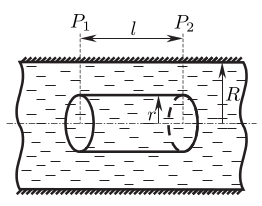
\includegraphics[scale=0.75]{theory.png}
    \caption{К выводу формулы Пуазейля}
\end{figure}

\begin{equation}
    F_\text{тр} = S \eta \frac{dv}{dr},
\end{equation}
где $S$ - площадь поверхности цилиндра, $\eta$ - вязкость,
$\frac{dv}{dr}$ - градиент скорости.

Теперь учтем нулевое ускорение тока, а также подставим $S = 2 \pi rl$

\begin{equation}
    (P_1 - P_2)\pi r^2 + 2 \pi rl \eta \frac{dv}{dr} = 0
\end{equation}
Проинтегрируем:

\begin{equation} \label{eqv}
    v = - \frac{P_1 - P_2}{4 \eta l}r^2 + C,
\end{equation}
где $C$ - константа интегрирования, которая должна быть найдена из граничных условий.
Воспользуемся фактом того, что жидкость у стенок сосуда обращается в нуль из-за трения:

\begin{equation}
    v = \frac{P_1 - P_2}{4\eta l}(R^2 - r^2)
\end{equation}
Теперь найдем расход жидкости, проинтегрировав сечение трубки по обручам:

\begin{equation} \label{eqQ}    
    Q = \frac{V}{t} = \int^R_0 2\pi r v dr = \pi \frac{P_1 - P_2}{8 \eta l} R^4
\end{equation}
Мы получили формулу Пуазейля. Но прежде чем её применять,
надо убедиться в ламинарности течения.
Ламинарное течение при переходе жидкости из широкого сосуда в капилляр
устанавливается не сразу, а после того, как она пройдет расстояние $a$:

\begin{equation} \label{eqa}
    a \approx 0.2R\cdot Re,
\end{equation}
где $R$ - радиус трубке, а $Re$ - число Рейнольдса

Формула \eqref{eqQ} работает, когда длина стержня много больше $a$.

\section{Измерение вязкости воды}

\subsection{Экспериментальная установка}

\begin{figure}[h]
    \centering
    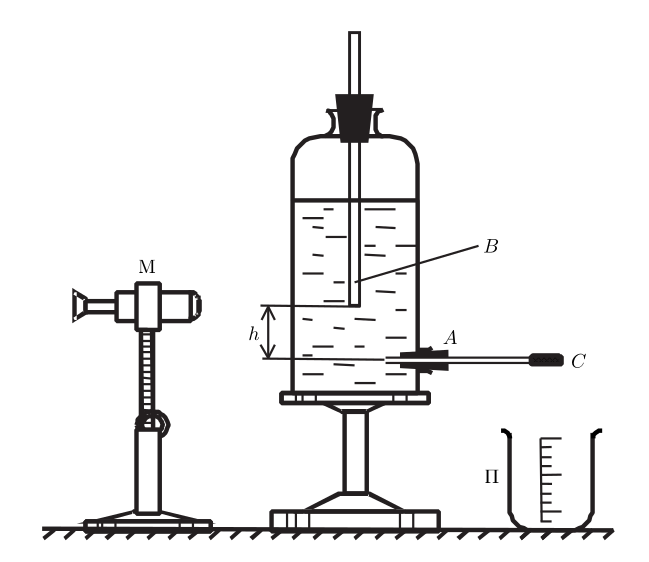
\includegraphics[scale=0.55]{A.png}
    \caption{Установка для определения вязкости воды}
\end{figure}

Для определения вязкости воды будем пользоваться формулой Пуазейля \eqref{eqQ}.
Воспользуемся сосудом Мариотта, чтобы поддерживать постоянную разность давлений. 
С помощью микроскопа на стенде с линейкой будем определять разность давлений.

\subsection{Обработка экспериментальных данных}

Экспериментально было выявлено влияния поверхностного натяжения на резутаты.
Выражается оно в том, что вода перестает вытекать при $h$ меньше некоторого $\Delta h$
Тогда и для давлений нужно сделать поправку $\Delta P = \rho g \Delta H$

До начала эксперимента также убедимся, что $a$ из формулы \eqref{eqa} много меньше длины стержня.

\begin{figure}[h]
    \centering
    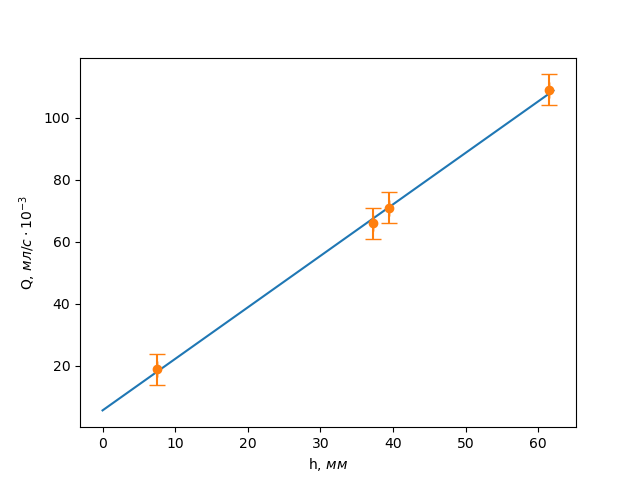
\includegraphics[scale=0.75]{graph_1.png}
    \caption{Зависимость расхода жидкости от разницы давления}
\end{figure}

Нанесем измерения на график, используя МНК, получим:

\begin{equation}
    \Delta h = (5.7 \pm 1.7) \ \text{мм}
\end{equation}

Непосредственное измерение дало результат:

\begin{equation}
    \Delta h_{ref} = (4.7 \pm 0.1) \ \text{мм}
\end{equation}

\begin{equation}
    \frac{dQ}{dh} = \frac{\rho g R^4}{8l} \cdot \frac{1}{\eta} = (1.66 \pm 0.09) \cdot 10^{-3}
                                                           \  \text{мл}/\text{c}
\end{equation}

Отсюда легко получить значения вязкости:

\begin{equation}
    \eta = (0.0093 \pm 0.0012) \text{П}
\end{equation}

При температуре $23^\circ C$ табличное значение вязкости:

\begin{equation}
    \eta_{ref} = 0.00936 \text{П}
\end{equation}

\newpage

\section{Измерение вязкости водного раствора глицерина \newline вискозиметром Оствальда}

\subsection{Установка}
            
\begin{wrapfigure}{r}{0.5\textwidth}
    \centering
    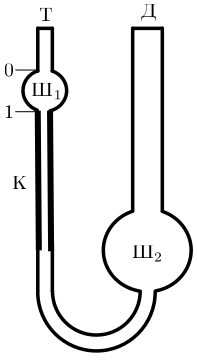
\includegraphics[width = 0.25\textwidth]{viski.png}
    \caption{Вискозиметр Оствальда}
\end{wrapfigure}

Вискозиметр Оствальда представляет собой U-образную стеклянную трубку.
Одно колено прибора в верхней части имеет расширение - шарик $\text{Ш}_1$ с метками
"0" и "1", и капилляр $K$. Другое колено представляет собой широкую трубку Д 
с резервуаром - шариком $\text{Ш}_2$

В широкую трубку вискозиметра вливают определенное количество воды, вязкость
которой известна. С помощью резиновой груши подсоединённой к узкой трубке Т,
в шарик засасывают воду. Затем, сняв грушу, засекают сколько воде требуется 
времени чтобы пройти от метки "0" до "1"

Для расчета процесса течения жидкости через капилляр воспользуемся формулой \eqref{eqQ}.
Разность давлений $P_1 - P_2$ постоянно меняется: значит, придется интегрировать:

\begin{equation}
    - \frac{dV}{dt} = \frac{\pi R^4}{8l} \frac{h(V) \rho \textsl{g}}{\eta},
\end{equation}
или иначе:

\begin{equation}
    -\frac{8l}{\pi R^4} \frac{dV}{h(V)} = \frac{\rho \textsl{g}}{\eta} dt
\end{equation}

Теперь проинтегрируем за время протекания воды отметок:

\begin{equation}
    \frac{8l}{\pi R^4} \int^{V_1}_{V_0} \frac{dV}{h(V)} =
                     - \int^{t_1}_{t_0} \frac{\rho \textsl{g}}{\eta} dt
\end{equation}

Заметим, что стоящая слева величина полностью зависит от параметров установки,
а значит можно получить:

\begin{equation}
    \frac{\rho t}{\eta} = const,
\end{equation}
или выразив вязкость искомой жидкости:

\begin{equation}
    \eta_x = \eta_0 \frac{\rho_x}{\rho_0} \frac{t_x}{t_0}
\end{equation}

Этой формулой мы и будем пользоваться на определения вязкости
10-, 20-, 30-процентых растворов глицерина.

\subsection{Обработка экспериментальных данных}

   \begin{table}[h]
    \centering
    \begin{center}
    \end{center}
    \vspace{0.05cm}
    \begin{tabular}{ |p{3cm}|p{3cm}|p{3cm}|p{3cm}| }
    \hline
    $\rho$ = 997.1 кг/м$^3$ & $\rho$ = 1019.2 кг/м$^3$ & $\rho$ = 1041.5 кг/м$^3$ & $\rho$ = 1064.6 кг/м$^3$\\
    \hline
     Вода, t, c & Глицерин 10\%, t, c & Глицерин 20\%. t, c & Глицерин 30\%, t, c \\ 
    \hline
    5.78 & 8.39 & 10.91 & 13.10\\
    5.85 & 8.46 & 10.87 & 13.04\\
    5.85 & 8.46 & 11.01 & 13.05\\
    5.90 & 8.29 & 10.80 & 13.00\\
    5.85 & 8.33 & 10.87 & 13.05\\
    
    \hline
    \hline
    
    $\bar t = 5.85$ с & $\bar t = 8.39$ с & $\bar t = 10.89$ с & $\bar t = 13.40$ с \\
    \hline
    $\sigma_t = 0.03$ c & $\sigma_t = 0.01$ c & $\sigma_t = 0.01$ c & $\sigma_t = 0.03$ c \\
    \hline
    \end{tabular}
    \caption{Время протекания жидкостей между метками}
    \end{table}

\newpage

\begin{equation}
    \eta_{ 0} = (9.3 \pm 1.2) \ \text{кП} \quad \ \eta_{ 0}^{ref} = 9.36 \ \text{кП}
\end{equation}
\begin{equation}
    \eta_{10} = (13.6 \pm 1.7) \ \text{кП} \quad \ \eta_{10}^ref = 13.1 \ \text{кП} 
\end{equation}
\begin{equation}
    \eta_{20} = (18 \pm 2) \ \text{кП} \quad \ \eta_{20}^ref = 17.7 \ \text{кП} 
\end{equation}
\begin{equation}
    \eta_{30} = (23 \pm 3) \ \text{кП} \quad \ \eta_{10}^ref = 25.0 \ \text{кП} 
\end{equation}


\section{Итоги}

Используя первую установку с сосудом Мариотта, мы смоги вычислить вязкость 
воды при комнатной температуре.
Благодаря второй установке с визкозиметром Оствальда мы смогли вычислить
вязкость 10-, 20-, 30-процентных растворов глицерина при комнатной температуре.

Все результаты совпали с табличными в пределах погрешности.
Однако погрешность получилась в районе $10\%-15\%$. 
Все потому что мы не можем измерить радиус трубки с большой точностью, а 
в формуле Пуазейля он стоит в 4 степени.

\newpage

\end{document}
